\documentclass[11pt]{standalone}
\usepackage{tikz}
\usetikzlibrary{shapes.geometric}
\usetikzlibrary{plotmarks,shapes.multipart}
\usetikzlibrary{arrows.meta,calc,decorations.pathmorphing}
\begin{document} 

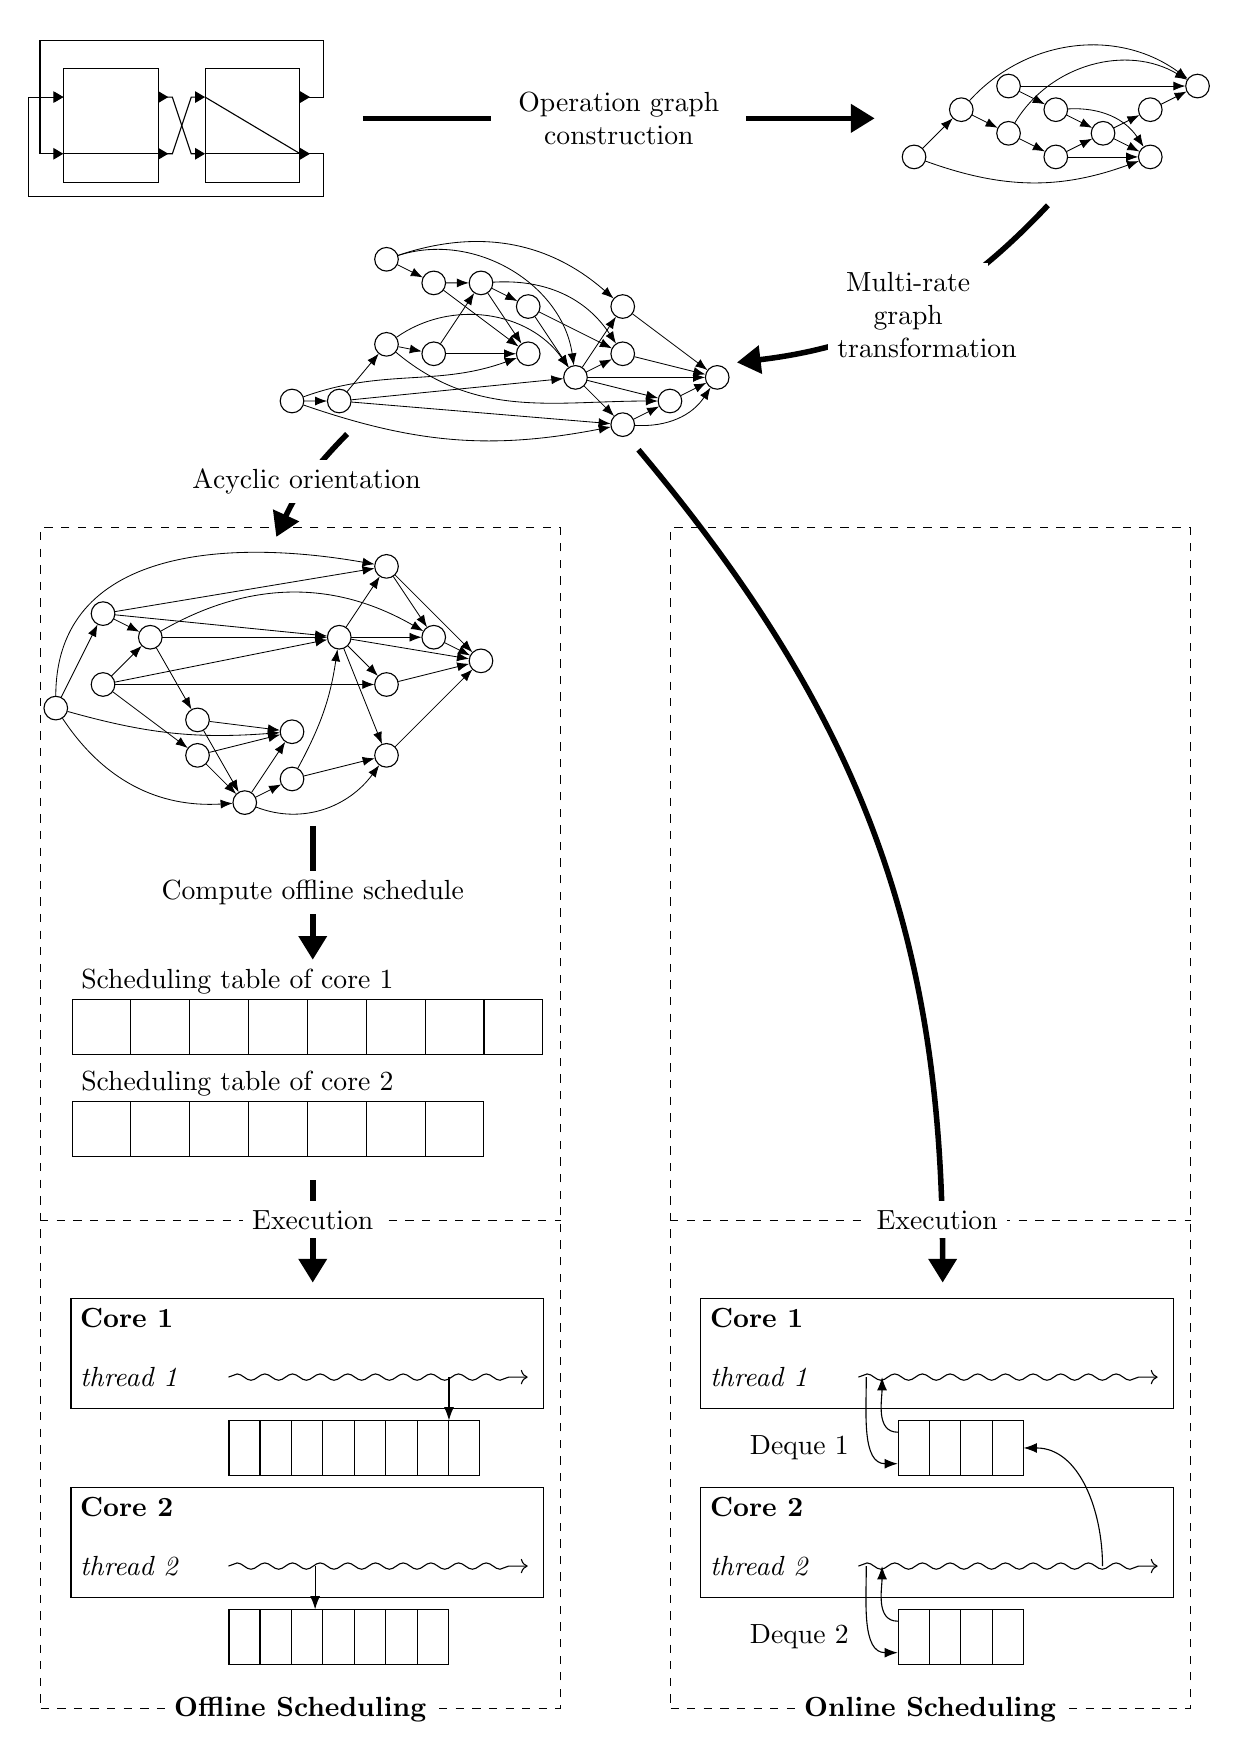
\begin{tikzpicture}
\begin{scope}[xshift=-2cm,yshift=.1cm,scale=.6,every node/.style={scale=0.6},local bounding box=scope1]
% FMU1
\node[rectangle,draw,minimum height = 2.4cm,minimum width = 2cm] (fmu1) {};

\draw[draw=white,-{Straight Barb[angle=60:2pt 3,black]}] ([yshift=0.6cm,xshift=-0.2cm]fmu1.west) -- ([yshift=0.6cm]fmu1.west);
%\draw[draw=white,-{Straight Barb[angle=60:2pt 3,black]}] ([yshift=-0.6cm,xshift=-0.2cm]fmu1.west) -- ([yshift=-0.6cm]fmu1.west);
\node[below of=fmu1,yshift=2.5cm] {};
\node[left of=fmu1,yshift=0.9cm,xshift=-0.2cm] {};
\node[left of=fmu1,yshift=-0.9cm,xshift=-0.2cm] {};
\node[right of=fmu1,yshift=0.9cm,xshift=0.2cm] {};
\node[right of=fmu1,yshift=-0.9cm,xshift=0.2cm] {};
\draw ([yshift=-0.6cm]fmu1.west) -- ([yshift=-0.6cm]fmu1.east);
% FMU2
\node[rectangle,draw,minimum height = 2.4cm,minimum width = 2cm, xshift=3cm] (fmu2) {};

\node[below of=fmu2,yshift=2.5cm] {};
\node[left of=fmu2,yshift=0.9cm,xshift=-0.2cm] {};
\node[left of=fmu2,yshift=-0.9cm,xshift=-0.2cm] {};
\node[right of=fmu2,yshift=0.9cm,xshift=0.2cm] {};
\node[right of=fmu2,yshift=-0.9cm,xshift=0.2cm] {};
\draw ([yshift=0.6cm]fmu2.west) -- ([yshift=-0.6cm]fmu2.east);
\draw ([yshift=-0.6cm]fmu2.west) -- ([yshift=-0.6cm]fmu2.east);

%Inter-FMU
\coordinate [right of =fmu2, yshift=1.8cm,xshift=.5cm] (c1);
\coordinate [left of =fmu1, yshift=1.8cm,xshift=-.5cm] (c2);

\coordinate [right of =fmu2, yshift=-1.5cm,xshift=.5cm] (c3);
\coordinate [left of =fmu1, yshift=-1.5cm,xshift=-.75cm] (c4);

\draw [-{Triangle[black]}]([yshift=0.6cm]fmu2.east) -| (c1) -- (c2) |- ([yshift=-.6cm]fmu1.west);
\draw [-{Triangle[black]}]([yshift=-.6cm]fmu2.east) -| (c3) -- (c4) |- ([yshift=.6cm]fmu1.west);

\coordinate [right of =fmu1, yshift=-.6cm,xshift=.3cm] (c5);
\coordinate [left of =fmu2, yshift=.6cm,xshift=-.3cm] (c6);

\coordinate [right of =fmu1, yshift=.6cm,xshift=.3cm] (c7);
\coordinate [left of =fmu2, yshift=-.6cm,xshift=-.3cm] (c8);

\draw [-{Triangle[black]}]([yshift=-.6cm]fmu1.east) -- (c5) -- (c6) -- ([yshift=.6cm]fmu2.west);
\draw [-{Triangle[black]}]([yshift=.6cm]fmu1.east) -- (c7) -- (c8) -- ([yshift=-.6cm]fmu2.west);

\draw[-{Triangle[black]},shorten >=-2pt] ([yshift=0.6cm]fmu1.east) -- ([yshift=0.6cm,xshift=0.09cm]fmu1.east);
\draw[-{Triangle[black]},shorten >=-2pt] ([yshift=-0.6cm]fmu1.east) -- ([yshift=-0.6cm,xshift=0.09cm]fmu1.east);

\draw[-{Triangle[]},shorten >=-2pt] ([yshift=0.6cm]fmu2.east) -- ([yshift=0.6cm,xshift=0.09cm]fmu2.east);
\draw[-{Triangle[]},shorten >=-2pt] ([yshift=-0.6cm]fmu2.east) -- ([yshift=-0.6cm,xshift=0.09cm]fmu2.east);

%\node[below of = fmu1,yshift=-1cm,xshift=1.5cm] {Co-simulation};
\end{scope}

\begin{scope}[xshift=10cm,scale=.6,every node/.style={scale=0.6},local bounding box=scope2]

%level 1
\node[circle,draw,minimum size=.5cm] at(-1,1) (o2) {};
\node[circle,draw,minimum size=.5cm] at(-3,-.5) (o6) {};
%level 3
\node[circle,draw,minimum size=.5cm] at(-1,0) (o3) {};
%level 5
\node[circle,draw,minimum size=.5cm] at(1,0) (o7) {};
%level 2
\node[circle,draw,minimum size=.5cm] at(0,.5) (o5) {};
\node[circle,draw,minimum size=.5cm] at(-2,.5) (o1) {};
%level 4
\node[circle,draw,minimum size=.5cm] at(0,-.5) (o4) {};
%level 6
\node[circle,draw,minimum size=.5cm] at(2,.5) (o0) {};
%level 7
\node[circle,draw,minimum size=.5cm] at(2,-.5) (o9) {};
\node[circle,draw,minimum size=.5cm] at(3,1) (o8) {};

%Inter-FMU
\draw [-{Latex[]},line width=.3pt] (o2) -- (o5);
\draw [-{Latex[]},line width=.3pt] (o3) -- (o4);
\draw [-{Latex[]},line width=.3pt] (o7) -- (o0);
\draw [-{Latex[]},line width=.3pt] (o6) -- (o1);

%Intra-FMU
\draw [-{Latex[]},line width=.3pt] (o1) -- (o3);
\draw [-{Latex[]},line width=.3pt] (o4) -- (o7);
\draw [-{Latex[]},line width=.3pt] (o5) -- (o7);

%To state
\path (o2) edge[-{Latex[]},line width=.3pt] (o8);
\path (o3) edge[-{Latex[]},bend left=45, line width=.3pt] (o8);
\path (o0) edge[-{Latex[]},line width=.3pt] (o8);
\draw (o1) edge[-{Latex[]},bend left=42,line width=.3pt] (o8);

\path (o4) edge[-{Latex[]},line width=.3pt] (o9);
\path (o5) edge[-{Latex[]},bend left,line width=.3pt] (o9);
\path (o6) edge[-{Latex[]},bend right=20,line width=.3pt] (o9);
\path (o7) edge[-{Latex[]},line width=.3pt] (o9);


%\node at(0,-1.6cm) {Operation graph};
\end{scope}

\begin{scope}[yshift=-2.5cm,xshift=3cm,scale=.6,every node/.style={scale=0.6},local bounding box=scope3]
%level 1
\node[circle,draw,minimum size=.5cm] at(-2.5,1.5) (o2) {};
\node[circle,draw,minimum size=.5cm] at(-4.5,-1.5) (o6) {};
%level 3
\node[circle,draw,minimum size=.5cm] at(-2.5,-.3) (o3) {};
%level 5
\node[circle,draw,minimum size=.5cm] at(-.5,1) (o7) {};
%level 2
\node[circle,draw,minimum size=.5cm] at(-1.5,1) (o5) {};
\node[circle,draw,minimum size=.5cm] at(-3.5,-1.5) (o1) {};
%level 4
\node[circle,draw,minimum size=.5cm] at(-1.5,-.5) (o4) {};
%level 6
\node[circle,draw,minimum size=.5cm] at(.5,.5) (o0) {};
%level 7
\node[circle,draw,minimum size=.5cm] at(.5,-.5) (o9) {};
\node[circle,draw,minimum size=.5cm] at(1.5,-1) (o8) {};

%Multirate nodes

\node[circle,draw,minimum size=.5cm] at(2.5,-.5) (o01) {};
\node[circle,draw,minimum size=.5cm] at(2.5,-2) (o11) {};
\node[circle,draw,minimum size=.5cm] at(2.5,.5) (o21) {};
\node[circle,draw,minimum size=.5cm] at(3.5,-1.5) (o31) {};
\node[circle,draw,minimum size=.5cm] at(4.5,-1) (o81) {};

%Inter-FMU
\draw [-{Latex[]},line width=.3pt] (o2) -- (o5);
\draw [-{Latex[]},line width=.3pt] (o3) -- (o4);
\draw [-{Latex[]},line width=.3pt] (o7) -- (o0);
\draw [-{Latex[]},line width=.3pt] (o6) -- (o1);

%Intra-FMU
\draw [-{Latex[]},line width=.3pt] (o1) -- (o3);
\draw [-{Latex[]},line width=.3pt] (o4) -- (o7);
\draw [-{Latex[]},line width=.3pt] (o5) -- (o7);

%To state
\path (o2) edge[-{Latex[]},bend left=50,line width=.3pt] (o8);
\path (o3) edge[-{Latex[]},bend left=45, line width=.3pt] (o8);
\path (o0) edge[-{Latex[]},line width=.3pt] (o8);
\draw (o1) edge[-{Latex[]},line width=.3pt] (o8);

\path (o4) edge[-{Latex[]},line width=.3pt] (o9);
\path (o5) edge[-{Latex[]},line width=.3pt] (o9);
\path (o6) edge[-{Latex[]},out=20,in=200,line width=.3pt] (o9);
\path (o7) edge[-{Latex[]},line width=.3pt] (o9);

%Multirate
\path (o6) edge[-{Latex[]},bend right=15,line width=.3pt] (o11);
\path (o1) edge[-{Latex[]},line width=.3pt] (o11);
\path (o7) edge[-{Latex[]},bend left,line width=.3pt] (o01);
\path (o0) edge[-{Latex[]},line width=.3pt] (o01);
\path (o8) edge[-{Latex[]},line width=.3pt] (o01);
\path (o8) edge[-{Latex[]},line width=.3pt] (o11);
\path (o2) edge[-{Latex[]},bend left,line width=.3pt] (o21);
\path (o3) edge[-{Latex[]},out=320,in=180,line width=.3pt] (o31);
\path (o8) edge[-{Latex[]},line width=.3pt] (o21);
\path (o8) edge[-{Latex[]},line width=.3pt] (o31);
\path (o8) edge[-{Latex[]},line width=.3pt] (o81);
\path (o01) edge[-{Latex[]},line width=.3pt] (o81);
\path (o11) edge[-{Latex[]},bend right,line width=.3pt] (o81);
\path (o21) edge[-{Latex[]},line width=.3pt] (o81);
\path (o31) edge[-{Latex[]},line width=.3pt] (o81);
\path (o11) edge[-{Latex[]},line width=.3pt] (o31);

%\node at(0,-2.6cm) {Operation graph};
\end{scope}

\begin{scope}[yshift=-7cm,scale=.6,every node/.style={scale=0.6},local bounding box=scope4]
%level 1
\node[circle,draw,minimum size=.5cm] at(-3.5,0) (o2) {};
\node[circle,draw,minimum size=.5cm] at(-4.5,-.5) (o6) {};
%level 3
\node[circle,draw,minimum size=.5cm] at(-2.5,1) (o3) {};
%level 5
\node[circle,draw,minimum size=.5cm] at(-.5,-2.5) (o7) {};
%level 2
\node[circle,draw,minimum size=.5cm] at(-1.5,-1.5) (o5) {};
\node[circle,draw,minimum size=.5cm] at(-3.5,1.5) (o1) {};
%level 4
\node[circle,draw,minimum size=.5cm] at(-1.5,-.75) (o4) {};
%level 6
\node[circle,draw,minimum size=.5cm] at(.5,-2) (o0) {};
%level 7
\node[circle,draw,minimum size=.5cm] at(.5,-1) (o9) {};
\node[circle,draw,minimum size=.5cm] at(1.5,1) (o8) {};

%Multirate nodes

\node[circle,draw,minimum size=.5cm] at(2.5,-1.5) (o01) {};
\node[circle,draw,minimum size=.5cm] at(2.5,2.5) (o11) {};
\node[circle,draw,minimum size=.5cm] at(2.5,0) (o21) {};
\node[circle,draw,minimum size=.5cm] at(3.5,1) (o31) {};
\node[circle,draw,minimum size=.5cm] at(4.5,.5) (o81) {};

%Inter-FMU
\draw [-{Latex[]},line width=.3pt] (o2) -- (o5);
\draw [-{Latex[]},line width=.3pt] (o3) -- (o4);
\draw [-{Latex[]},line width=.3pt] (o7) -- (o0);
\draw [-{Latex[]},line width=.3pt] (o6) -- (o1);

%Intra-FMU
\draw [-{Latex[]},line width=.3pt] (o1) -- (o3);
\draw [-{Latex[]},line width=.3pt] (o4) -- (o7);
\draw [-{Latex[]},line width=.3pt] (o5) -- (o7);

%To state
\path (o2) edge[-{Latex[]},line width=.3pt] (o8);
\path (o3) edge[-{Latex[]}, line width=.3pt] (o8);
\path (o0) edge[-{Latex[]},bend right=10,line width=.3pt] (o8);
\draw (o1) edge[-{Latex[]},line width=.3pt] (o8);

\path (o4) edge[-{Latex[]},line width=.3pt] (o9);
\path (o5) edge[-{Latex[]},line width=.3pt] (o9);
\path (o6) edge[-{Latex[]},bend right=10,line width=.3pt] (o9);
\path (o7) edge[-{Latex[]},line width=.3pt] (o9);

%Multirate
\path (o6) edge[-{Latex[]},out=90,in=170,looseness=1.1,line width=.3pt] (o11);
\path (o1) edge[-{Latex[]},line width=.3pt] (o11);
\path (o7) edge[-{Latex[]},bend right=35,out=320,line width=.3pt] (o01);
\path (o0) edge[-{Latex[]},line width=.3pt] (o01);
\path (o8) edge[-{Latex[]},line width=.3pt] (o01);
\path (o8) edge[-{Latex[]},line width=.3pt] (o11);
\path (o2) edge[-{Latex[]},line width=.3pt] (o21);
\path (o3) edge[-{Latex[]},bend left, line width=.3pt] (o31);
\path (o8) edge[-{Latex[]},line width=.3pt] (o21);
\path (o8) edge[-{Latex[]},line width=.3pt] (o31);
\path (o8) edge[-{Latex[]},line width=.3pt] (o81);
\path (o01) edge[-{Latex[]},line width=.3pt] (o81);
\path (o11) edge[-{Latex[]},line width=.3pt] (o81);
\path (o21) edge[-{Latex[]},line width=.3pt] (o81);
\path (o31) edge[-{Latex[]},line width=.3pt] (o81);
\path (o11) edge[-{Latex[]},line width=.3pt] (o31);

% Orientation
\path (o6) edge[-{Latex[]},bend right,line width=.3pt] (o7);
\path (o2) edge[-{Latex[]},line width=.3pt] (o3);

%\node at(0,-3cm) {Operation graph};
\end{scope}

\begin{scope}[shift={($(scope4.north)+(-1.5,1cm)$)},local bounding box=scope5]
% Compute Schedule
\node at(-1cm,0) [rectangle split,rectangle split horizontal,rectangle split parts=8,text width=.5cm,anchor=west, draw, minimum width=6cm,minimum height=.7cm,yshift=-7.2cm,label={[anchor=north west, yshift=.5cm]north west:{Scheduling table of core 1}}]{\hfil \nodepart{two}\hfil \nodepart{three}\hfil \nodepart{four}\hfil \nodepart{five}\hfil \nodepart{six}\hfil \nodepart{seven}\hfil \nodepart{eight}\hfil};
\node at(-1cm,0) [rectangle split,rectangle split horizontal,rectangle split parts=7,text width=.5cm,anchor=west, draw, minimum width=6cm,minimum height=.7cm,yshift=-8.5cm,,label={[anchor=north west, yshift=.5cm]north west:{Scheduling table of core 2}}]{\hfil \nodepart{two}\hfil \nodepart{three}\hfil \nodepart{four}\hfil \nodepart{five}\hfil \nodepart{six}\hfil \nodepart{seven}\hfil};
\end{scope}

\begin{scope}[shift={($(scope5.north)+(0,1cm)$)},local bounding box=scope6]
% Execute
\node at(0cm,-6cm) [rectangle, draw, minimum width=6cm,minimum height=1.4cm,label={[anchor=north west, yshift=-.01cm]north west:{\textbf{Core 1}}},label={[anchor=west, yshift=-.3cm]west:{\textit{thread 1}}}] {};
\node at(-1cm,0) [rectangle split,rectangle split horizontal,rectangle split parts=8,anchor=west, draw, minimum width=5.6cm,minimum height=.7cm,yshift=-7.2cm]{};
\draw [->,decorate,decoration={snake,pre=curveto,pre length=1,post length=1,amplitude=.4mm}] (-1cm,-6.3cm) -- (2.8cm,-6.3cm);
\draw [-{Latex[]}] (1.8cm,-6.3cm) -- (1.8cm,-6.85cm);

\node at(0cm,-8.4cm) [rectangle, draw, minimum width=6cm,minimum height=1.4cm,label={[anchor=north west, yshift=-.01cm]north west:{\textbf{Core 2}}},label={[anchor=west, yshift=-.3cm]west:{\textit{thread 2}}}]{};
\node at(-1cm,0) [rectangle split,rectangle split horizontal,rectangle split parts=7,anchor=west, draw, minimum width=5.6cm,minimum height=.7cm,yshift=-9.6cm]{};
\draw [->,decorate,decoration={snake,pre=curveto,pre length=1,post length=1,amplitude=.4mm}] (-1cm,-8.7cm) -- (2.8cm,-8.7cm);
\draw [-{Latex[]}] (.1cm,-8.7cm) -- (.1cm,-9.25cm);

\end{scope}

\begin{scope}[shift={($(scope5.north)+(8cm,1cm)$)},local bounding box=scope7]
\node at(0cm,-6cm) [rectangle, draw, minimum width=6cm,minimum height=1.4cm,label={[anchor=north west, yshift=-.01cm]north west:{\textbf{Core 1}}},label={[anchor=west, yshift=-.3cm]west:{\textit{thread 1}}}] {};
\node at(-.5cm,0) [rectangle split,rectangle split horizontal,rectangle split parts=4,anchor=west, draw, minimum width=5.6cm,minimum height=.7cm,yshift=-7.2cm,label={[anchor=east, xshift=-.5cm]west:{Deque 1}}](deque1){};
\draw [->,decorate,decoration={snake,pre=curveto,pre length=1,post length=1,amplitude=.4mm}] (-1cm,-6.3cm) -- (2.8cm,-6.3cm);
\path ([yshift=.2cm]deque1.west) edge[-{Latex[]},in=270,out = 180,looseness=1]  (-.7cm,-6.3cm);
\path (-.9cm,-6.3cm) edge[-{Latex[]},out=270,in = 180,looseness=1] ([yshift=-.2cm]deque1.west);

\node at(0cm,-8.4cm) [rectangle, draw, minimum width=6cm,minimum height=1.4cm,label={[anchor=north west, yshift=-.01cm]north west:{\textbf{Core 2}}},label={[anchor=west, yshift=-.3cm]west:{\textit{thread 2}}}]{};
\node at(-.5cm,0) [rectangle split,rectangle split horizontal,rectangle split parts=4,anchor=west, draw, minimum width=5.6cm,minimum height=.7cm,yshift=-9.6cm,label={[anchor=east, xshift=-.5cm]west:{Deque 2}}](deque2){};
\draw [->,decorate,decoration={snake,pre=curveto,pre length=1,post length=1,amplitude=.4mm}] (-1cm,-8.7cm) -- (2.8cm,-8.7cm);
\path ([yshift=.2cm]deque2.west) edge[-{Latex[]},in=270,out = 180,looseness=1]  (-.7cm,-8.7cm);
\path (-.9cm,-8.7cm) edge[-{Latex[]},out=270,in = 180,looseness=1] ([yshift=-.2cm]deque2.west);

\path (2.1cm,-8.7cm) edge[-{Latex[]},out=90,in = 0,looseness=1] (deque1.east);

\end{scope}

%\draw [dashed] (4.5,-6cm) -- (4.5,-22.7cm);
\path ([xshift=.5cm]scope1.east) edge[-{Triangle[]},line width=2pt, midway,text width = 3cm,align = center] node[fill=white]{Operation graph construction} ([xshift=7cm]scope1.east);

\path ([xshift=-.1cm,yshift=-.2cm]scope2.south) edge[-{Triangle[]},line width=2pt, bend left=20,midway,text width = 1.8cm,align = center] node[fill=white]{Multi-rate graph \mbox{transformation}} ([xshift=.1cm,yshift=-.3cm]scope3.east);

\path ([xshift=-2cm,yshift=.2cm]scope3.south) edge[-{Triangle[]},line width=2pt, bend right=10,midway,text width = 3.8cm,align = center] node[fill=white]{Acyclic orientation} ([xshift=.1cm,yshift=.02cm]scope4.north);

\path ([xshift=.07cm,yshift=1.7cm]scope5.north) edge[-{Triangle[]},line width=2pt,midway,align = center] node[fill=white]{Compute offline schedule} ([xshift=.07cm,yshift=0cm]scope5.north);

\path ([xshift=.07cm,yshift=1.5cm]scope6.north) edge[-{Triangle[]},line width=2pt,midway,align = center] node{} ([xshift=.07cm,yshift=.2cm]scope6.north);

\path ([xshift=1.7cm,yshift=0cm]scope3.south) edge[-{Triangle[]},bend left = 20,line width=2pt,midway,align = center] node{} ([xshift=.07cm,yshift=.2cm]scope7.north);%([xshift=.07cm]exec2.north);
%\draw [-{Triangle[]},line width=2pt] ([xshift=.07cm]exec2.south) -- ([xshift=.07cm,yshift=.2cm]scope7.north);

\node at (-2.9cm,-5cm)[anchor= north west,rectangle,draw,dashed,minimum height=15cm,minimum width=6.6cm] (frame1) {};
\node [anchor= north west,rectangle,draw,dashed, right of = frame1, minimum height=15cm,minimum width=6.6cm,xshift=7cm] (frame2) {};

\node at(frame1.south) [fill=white] {\textbf{Offline Scheduling}};
\node at(frame2.south) [fill=white] {\textbf{Online Scheduling}};

\draw [dashed] ([yshift=-1.3cm]frame1.west) -- ([yshift=-1.3cm]frame1.east);
\draw [dashed] ([yshift=-1.3cm]frame2.west) -- ([yshift=-1.3cm]frame2.east);

\node [fill=white] at([xshift=.07cm,yshift=1cm]scope6.north) {Execution};
\node [fill=white] at([yshift=1cm]scope7.north) (exec2){Execution};


\end{tikzpicture}
\end{document}